\documentclass[11pt, a4paper]{article}
\usepackage[utf8]{inputenc}
\usepackage[ngerman]{babel}
\usepackage{graphicx}
\usepackage{listings}

\begin{document}

\tableofcontents
\thispagestyle{empty}
\newpage

\section{Einleitung}
Hier eine kurze Einleitung in welchem Rahmen diese Arbeit entstanden ist und schonmal ganz kurz auf SETI eingehen.

\section{SETI Breakthrough Listen}
Die kaggle Challenge SETI Breakthrough Listen - E.T. Signal Search war ein öffentlicher Machine Learning Wettbewerb des Berkeley SETI Research Centers im Zeitraum vom 10. Mai 2021 bis 18. August 2021. Die zugrunde liegenden Daten sind noch verfügbar, sodass Interessierte sich nach wie vor mit diesem Problem beschäftigen können. Im folgenden werden wir die Challenge stets abgekürzt als SETI bezeichnen. 

Die Herausforderung bei SETI besteht darin, Spektrogramme, also eine bildliche Darstellung eines Frequenzbereichs in einem bestimmten Zeitraum, die basierend auf Rohdaten des Green Bank Telescopes generiert worden sind, auf das Vorkommen von künstlich hinzugefügten extraterrestrischen Signalen zu untersuchen. Hierbei ist es wichtig, diese Signale von irdisches Signalen, wie etwa einem Radiosignal, zu unterscheiden. Um diese Unterscheidung vornehmen zu können, sind jeweils sechs Spektrogramme zusammengefasst, wobei die Spektrogramme eins, drei und fünf jeweils Aufnahmen des zu untersuchenden Ziels \glqq A\grqq{} sind und die übrigen jeweils auf Aufnahmen eines anderen Himmelskörpers \glqq B\grqq{}, \glqq C\grqq{} und \glqq D\grqq{}. Eine solche Gruppe von Spektrogrammen (ABACAD) wird bei \emph{SETI} als \emph{Kadenz-Ausschnitt}, im folgenden nur noch \glqq Kadenz\grqq{}, bezeichnet.

Abbildung \ref{fig:kadenz_pos_1} zeigt ein Beispiel für eine Kadenz mit einem extraterrestrischen Signal. Auf den drei Spektrogrammen, die auf das Ziel gerichtet sind (in der Abbildung durch \glqq ON\grqq{} gekennzeichnet) ist jeweils ein Signal zu erkennen, welches nicht auf den anderen Spektrogrammen zu sehen ist. Offensichtlich muss ein Signal nicht auf jedem der drei \emph{on target} Spektrogrammen zu sehen sein, da ein Signal nicht zwingend über den gesamten zeitlichen Betrachtungsraum aktiv sein muss.

\begin{figure}[t]
\centering
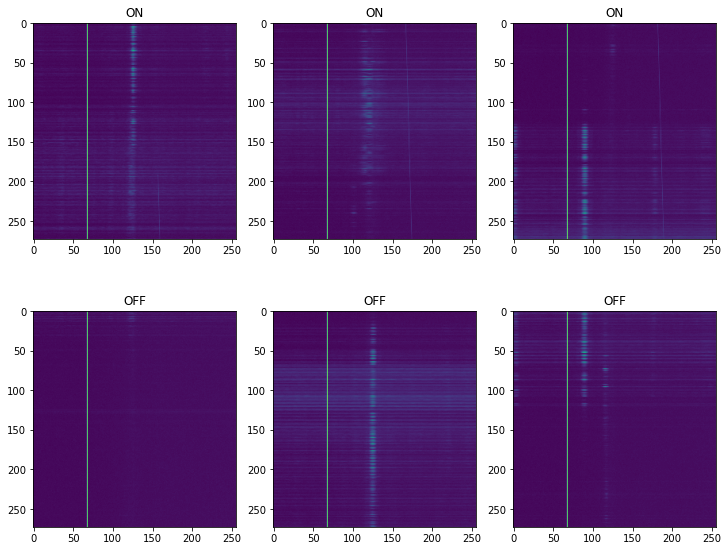
\includegraphics[width=0.9\textwidth]{"img/kadenz_pos_1.png"}
\caption{Beispiel für eine Kadenz mit Nadel}
\label{fig:kadenz_pos_1}
\end{figure}

Die Trainingsdaten für \emph{SETI} enthalten 60.000 Kadenzen (\emph{Heuhaufen}) von denen 6.000 \emph{Nadeln} sind, also Kadenzen, die ein künstlich eingefügtes extraterrestrisches Signal enthalten. Einige dieser Signale sind bei entsprechender Visualisierung sofort mit bloßem Auge zu erkennen, andere sind in, durch irdische Signale verursachten, Rauschen versteckt. Weil die Challenge zum Zeitpunkt der Projektarbeit nicht mehr aktiv ist und die zu den Testdaten der Challenge keine Labels verfügbar sind, müssen wir die Trainingsdaten in Trainings- und Testdaten aufteilen, um ein Modell abschließend auf Testdaten laufen lassen zu können. Hierzu führen wir einen 70/30 Split der Trainingsdaten durch und erhalten danach ein Trainingsset mir 42000 Kadenzen und ein Testset mit 18000 Kadenzen. Dieser Split wird durch einen \emph{Seed} reproduzierbar gemacht, um verschiedene Modelle vergleichen zu können, in dem sie auf dem jeweils selben Split der verfügbaren Daten trainiert und getestet werden.


\section{Implementierung}
Im folgenden beschäftigen wir uns nun mit der Problemlösung für \emph{SETI}. Wir schauen uns erste Ansätze mit reiner Computer Vision an, die uns helfen sollen auch versteckte Signale extrahieren zu können, um sie mit bloßem Auge erkennen zu können. Wir haben uns für diesen Einstieg entschieden, um ein Gefühl für die visuelle Form der gesuchten Signale und für den Datensatz allgemein zu erhalten. Im darauf folgenden Kapitel werden wir uns mit \emph{Convulutional Neural Networks}, kurz \emph{CNNs}, beschäftigen.

\subsection{Erste Ansätze mit Computer Vision}
Wenn man über Bilderkennung spricht denkt man meistens direkt an Machine Learning und Neurale Netzwerke. Allerdings gibt es in der Bilderkennung Problematiken, die sich mithilfe der klassischen Computer Vision deutlich besser lösen lassen. Im Folgenden wird auf die grundlegenden Unterschiede zwischen der klassischen Computervision und Machine Learning eingegangen, einige Grundlagen beschrieben, Lösungen der Computervision angewandt auf die Problematik der Projektarbeit und ob die klassische Computervision für diese Projektarbeit geeignet ist.

\subsubsection{Unterschiede Computervision - Machine Learning}
Computervision ist nicht gleichzusetzen mit Machine Learning. Die klassische Computervision arbeitet mit rein mathematischen Ansätzen und Algorithmen, während das klassische Machine Learning eher darauf bedacht ist mithilfe von Trainingsdaten Modelle zu trainieren und dadurch Parameteranpassungen durchzuführen. Computervision ist sehr vielfältig einsetzbar. Mithilfe von Algorithmen können beispielsweise alle möglichen geometrische Primitive detektiert werden, also beispielsweise Linien und Kreise. Außerdem kann mithilfe von sogenannten Filtern das Bild verarbeitet werden um zum Beispiel bestimmte Elemente im Bild zu eleminieren, das Bild zu schärfen oder zu glätten und noch vieles darüber hinaus. Diese Filter werden außerdem in den nachfolgenden Kapiteln noch sehr interessant für die Convolutional Neural Networks.

\subsubsection{Grundlagen}
Bilder sind im Prinzip nichts weiter als eine große Ansammlung von Zahlen, welche die entsprechenden Farben repräsentieren. In der klassischen Computervision arbeitet man häufig mit sogenannten Grauwertbildern. Diese sind besonders einfach zu handhaben, da diese nur einen Farbkanal besitzen im Gegensatz zu RGB Farbbildern, welche die 3 Farbkanäle Rot, Grün und Blau besitzen.

\subsubsection{Lokale Operatoren: Filter}
Lokale Operatoren sind sogenannte Punktoperationen, also Operationen die auf jedem Pixel des Bildes angewandt werden. Bei Lokalen Operatoren ist die Besonderheit, dass benachbarte Pixel auch mit in die Berechnung der Operation einfließen und somit auch den Farbwert des betrachteten Pixels beeinflussen. Somit können zum Beispiel Grauwertübergänge, also Übergänge von dunkel nach hell, detektiert werden. Um Punktoperationen besser zu verstehen, muss man das Bild als eine drei-dimensionale Funktion betrachten: die x Achse steht für die Breite des Bildes, y ist die Höhe des Bildes und z die Farbe des entsprechenden Pixels an der Stelle (x,y), so erhält man eine Grauwertfunktion g(x,y)=z. An den Stellen wo es einen schnellen Wechsel von dunkel zu hell gibt, hat die Ableitung der Grauwertfunktion einen Extrempunkt. Die Ableitung der Grauwertfunktion lautet:
\newline

g'(x,y)=[$\frac{\partial g(x,y)}{\partial x}$, $\frac{\partial g(x,y)}{\partial y}$]$^T$
\newline
Für diskrete Bilder muss die Ableitung allerdings angenähert werden, da ein Pixel nur einen einzigen Wert beinhaltet:
\newline

$\frac{\partial g(x,y)}{\partial x}$ = $\frac{g(x+\Delta x,y)-g(x-\Delta x,y)}{\Delta x}$
\newline

$\frac{\partial g(x,y)}{\partial y}$ = $\frac{g(x,y+\Delta y)-g(x,y-\Delta y)}{\Delta y}$
\newline
Setzt man nun $\Delta x$ beziehungsweise $\Delta y$ gleich 1 erhält man folgende Approximationen:
\newline

$\frac{\partial g(x,y)}{\partial x}$ = $\frac{g(x+1,y)-g(x-1,y)}{1}$
\newline

$\frac{\partial g(x,y)}{\partial y}$ = $\frac{g(x,y+1)-g(x,y-1)}{1}$
\newline
Für jedes Pixel (x,y) auf welches diese Approximation angewandt wird, wird also folgendes berechnet:
\newline

$1\cdot g(x+1,y)+0\cdot g(x,y)-1\cdot g(x-1,y)$
\newline
Wir erhalten also folgendes Operatorfenster:
\begin{figure}[h]
\centering
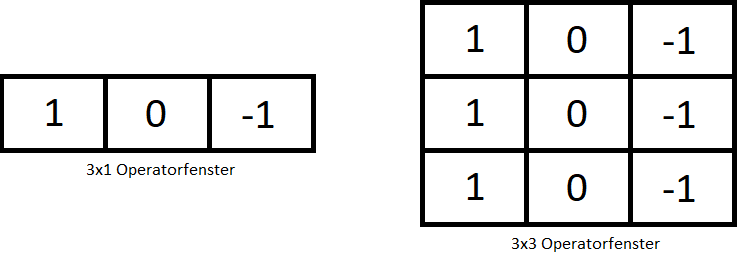
\includegraphics[width=0.9\textwidth]{img/operatorfenster.png}
\end{figure}
\newline
Mit dem Operatorfenster kann auf jedem einzelnen Pixel eine sogenannte gewichtete Addition ausgeführt werden, was genau der oben hergeleiteten Berechnungen entspricht. Dafür legt man das Operatorfenster auf eine entsprechende Stelle des Bildes, multipliziert die einzelnen Komponenten des Fensters mit den darunterliegenden Werten der Pixel und summiert diese Produkte. Anstatt eines 3x1 Operatorfensters können auch 3x3 Operatorfenster genutzt werden, wodurch auch Pixel die über und unter dem zu betrachtenden Pixel mit in die Berechnung einfließen. Das Ergebnis der Anwendung des oben abgebildeten Operatorfensters ist ein neues Bild, welches insbesondere vertikale Grauwertübergänge hervorhebt und horizontale Grauwertübergänge entfernt. Der Grund dafür ist die Approximation der ersten Ableitung in x-Richtung, wodurch die Grauwertfunktion des Bildes abgeleitet wird. Dadurch kann man das resultierende Bild sozusagen als Ableitung des Originalgrauwertbildes betrachten: Stellen die hervorgehoben werden, sind starke Grauwertübergänge und horizontale Linien werden entfernt, da auf einer gleichfarbigen horizontalen Linie keine ausschlaggebenden Veränderungen der Grauwerte vorkommen. Dasselbe gilt umgekehrt für die Approximation in y-Richtung - dafür muss das Operatorfenster einfach nur um 90 Grad gedreht werden. Mit der Approximation in y-Richtung werden allerdings vertikale Linien eleminiert.
\begin{figure}[h]
\centering
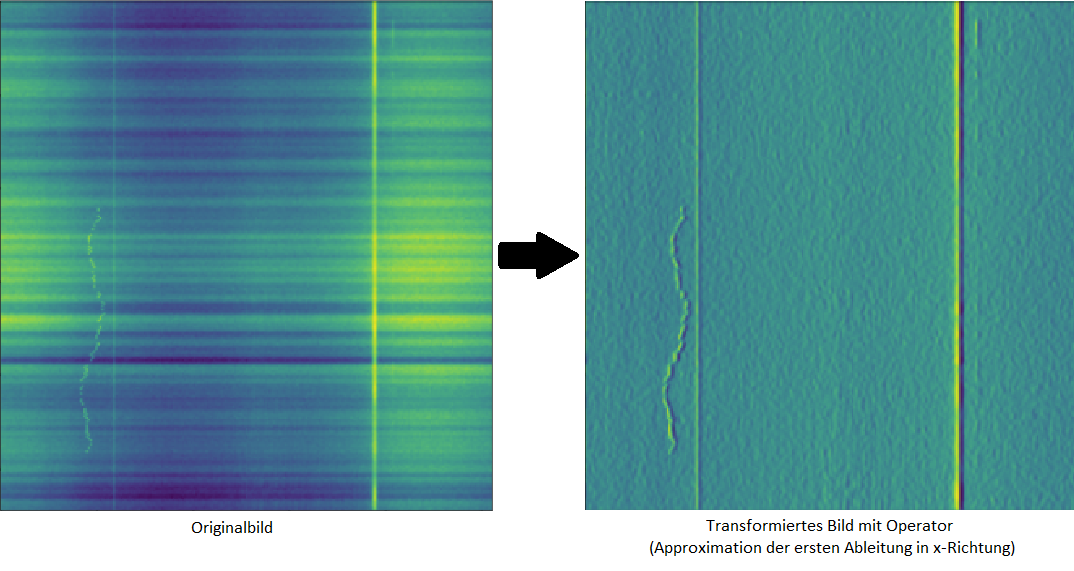
\includegraphics[width=0.9\textwidth]{img/original-vs-cv.png}
\end{figure}
\newline
Die Idee hinter der Verwendung der Filter ist die, dass die Signale alle eine vertikale Richtung aufweisen. Mithilfe der Filter für die Eleminierung der horizontalen Linien kann also Rauschen recht einfach rausgefiltert werden.
TODO: Referenz auf Laubenheimer Folien

\subsubsection{Weitere Experimente}
Das Rauschen in den Bildern ist häufig sehr ausgeprägt, weshalb auch mit Algorithmen zur Rauschminderung experimentiert wurde. Die Idee hinter dem ersten Algorithmus war es ähnliche Pixel auf dieselbe Farbe abzubilden. Anfangs wird die Anzahl der unterschiedlichen Farben gezählt und anschließend die mittlere Differenz der Farbwerte berechnet. Anhand der mittleren Differenz und ein als Parameter festgelegter Wert, der bestimmt wie stark die mittlere Differenz den Algorithmus beeinflusst, kann ein neuer Wert berechnet werden, der bestimmt wie unterschiedlich ähnliche Pixel zueinander sein dürfen, sodass sie auf dieselbe Farbe abgebildet werden. 
\newline
Nachdem nun dieser Algorithmus zur Abbildung ähnlicher Pixel auf dieselbe Farbe angewandt wurde, kann es sein dass die unterschiedlichen Farben teilweise einen geringeren, aber auch einen höheren Abstand zum jeweils nächsten Farbwert haben. Die Lösung dafür ist genau diese Differenz zwischen allen Farbwerten auf die mittlere Differenz zu setzen. Dadurch erreicht man, dass die Farben, die bislang noch sehr nah beieinander lagen, nach Anwendung dieses Algorithmus besser zu unterscheiden sind und Farben, die bislang eher weiter weg voneinander lagen, immer noch gut voneinander unterscheidbar sind. Anfangs wird wieder die Anzahl der unterschiedlichen Farben gezählt und auch die mittlere Differenz zwischen den einzelnen Farben berechnet. Da die Farben nach Anwendung des Algorithmus genau diese mittlere Differenz zueinander haben soll, werden die Farben nacheinander auf jeweils ein Vielfaches der mittleren Farbdifferenz abgebildet.
\newline
Führt man vor diesen beiden Algorithmen den Filter zur Entfernung der horizontalen Linien aus, erhält man beispielsweise folgende Transformation:
\begin{figure}[h]
\centering
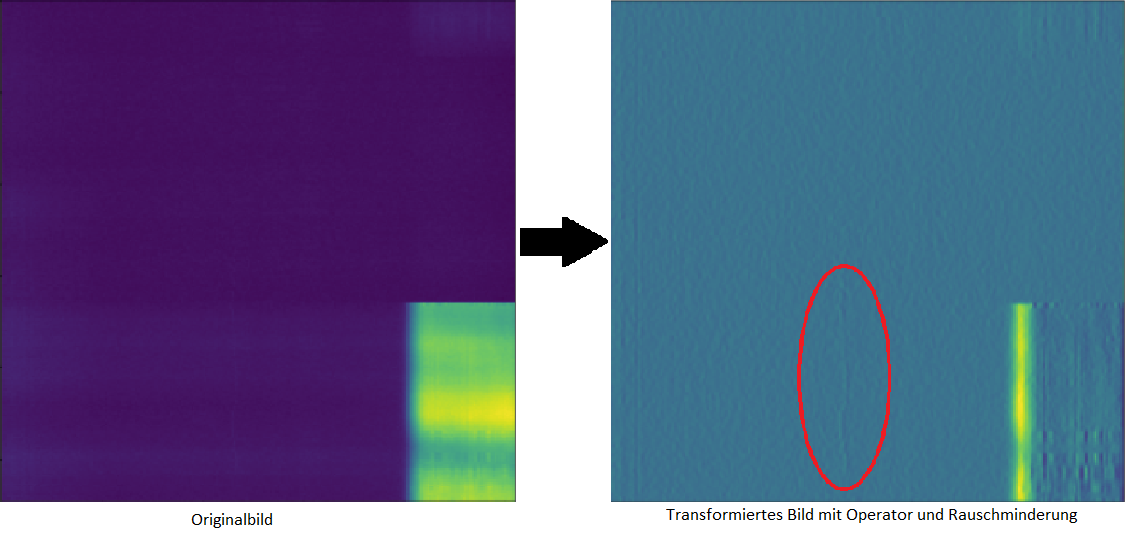
\includegraphics[width=0.9\textwidth]{img/original-vs-rauschminderung.png}
\end{figure}
\newline
Auf dem Originalbild ist mit dem bloßen Auge kein Signal zu finden, betrachtet man allerdings das transformierte Bild ist ein schwaches Signal zu erkennen.

\subsubsection{Zwischenfazit: Computervision alleine bringt keinen Erfolg}
Computervision ist zwar sehr vielfältig einsetzbar, allerdings für die Problematik dieser Projektarbeit nur sehr schwer anwendbar. Das liegt insbesondere daran, dass die Signale teilweise im Hintergrundrauschen sehr gut versteckt sind und teilweise nicht mal mit dem Auge zu erkennen sind. Wie bereits erläutert, kann man zwar mithlife von Filtern und etwas Algorithmik die Signale besser vom Hintergrund hervorheben, allerdings müssten die Signale für eine reine Computervision Lösung detektierbar sein. Dafür hat die Computervision wie bereits am Anfang erwähnt zum Beispiel Möglichkeiten für die Detektion von geometrischen Primitiven. Allerdings sind viele der Signale auch nach Verarbeitung der Algorithmen nur schwer zu erkennen und darüberhinaus ist die Form der Signale unbestimmt, was die Detektion auf Basis von Algorithmen sehr schwer macht. Eine andere Möglichkeit der Detektion ist die Anwendung von Convolutional Neural Networks, worauf in dem nächsten Kapitel näher eingegangen wird.

\section{Deep Learning}
Natürlich wollen wir nicht alle Kadenzen einzeln manuell betrachten und entscheiden, ob sie eine Nadel enthalten oder nicht. Vielmehr wollen wir ein Machine Learning Model trainieren, das uns diese Arbeit abnimmt und Nadeln findet. Hierzu wollen wir ein Convolutional Neural Network (CNN) trainieren, das die Kadenzen in genau zwei Klassen einteilt: enthält eine Nadel oder enthält keine Nadel.

\subsection{Das erste Convolutional Neural Network}
Um uns an den Umgang mit CNNs heranzutasten, entwerfen wir zunächst ein kleines Netz bestehend aus zwei Hidden Layern und einem Fully Connected Layer. Die beiden Hidden Layer bestehen aus je einem Convolutional Layer und einem Pooling Layer. Wir teilen die Trainingsdaten noch einmal mit einem Verhältnis von 90 zu 10 in Trainings- und Validierungsdaten. 

Unsere erste Beobachtung ist, dass wir selbst mit einem so kleinen Netz bereits eine sehr hohe Accuracy erzielen und sich auch der Loss am Anfang deutlich verringert, bis er ein Plateau erreicht. Jedoch ist der Recall sehr schlecht. Diese Konstellation der Metriken lässt sich damit erklären, dass unser CNN nicht wirklich gelernt hat, wie die gesuchten Signale aussehen, sondern einfach die meisten Kadenzen der Klasse 0, also enthält keine Nadel, zuordnet. Aufgrund des sehr unbalancierten Datensatzes, ist diese Klassifizierung offensichtlich sehr oft richtig und somit kommt es zu einem hohen Accuracy Score. Der niedrige Wert beim Recall zeigt jedoch, dass unser Modell die Nadeln nur äußerst selten erkennt. Wir fügen nun weitere Hidden Layer hinzu und spielen viel mit den Werten für die Hyperparameter Kernel Size, Padding und Output Channels. Im Wesentlichen bleibt die Beobachtung jedoch gleich. Das Modell erkennt die Nadeln nur selten.

\subsection{Transfer Learning}
Wir stehen nun vor der Wahl das eigene CNN weiter auszubauen oder ein vortrainiertes CNN zu verwenden. Beim Transfer Learning wird gewonnenes Wissen aus ähnlichen Aufgaben für die aktuelle Aufgabe genutzt. Für die Klassifizierung von Bildern können wir auf ein vortrainiertes Convolutional Neural Network zurückgreifen, dass beispielsweise bereits auf den Daten von ImageNet, einem riesigen Datensatz mit Millionen von Bildern, trainiert worden ist.

\subsubsection{EfficientNet}
Wir entscheiden uns EfficientNet als Grundlage für unsere weiteren Versuche zu verwenden. EfficientNet ist ein sehr beliebtes Modell im Bereich der Bildklassifizierung und erzielt auf den ImageNet Daten sehr gute Ergebnisse. PyTorch stellt einige Varianten des EfficientNets bereit und wir trainieren einige dieser Varianten auf den SETI Daten. Das  

\subsection{Imbalance}
Unter Imbalanced Datasets, also unausgeglichenen Datensätzen, versteht man die Problematik, dass mindestens ein Label in einem Datensatz häufiger vertreten ist als andere Labels. Das Problem bei Imbalanced Datasets ist, dass das Modell mehr darauf trainiert wird die häufiger vorkommenden Labels zu erkennen, da entsprechende Labels öfter vom Modell gesehen werden und entsprechend stärker das Modell beeinflussen als andere Labels. Für diese Problematik gibt es einige Lösungsansätze:
\newline
Oversampling ist eine hervorragende Lösung um aus einem imbalanced Dataset ein balanced Dataset zu erschaffen. Dabei werden die weniger vorkommenden Labels entsprechend zufällig vervielfacht um ein ausgewogenes Verhältnis zwischen allen Labels zu schaffen. Natürlich gibt es noch einige weitere Strategien zum Beispiel das genaue Gegenteil von Oversampling: das Undersampling. Es werden zufällig Daten von den häufig vorkommenden Labels aus dem Datensatz entfernt. Eine andere Strategie setzt bei der Loss-Berechnung an: Die Gewichtung der entsprechenden Labels kann in der Berechnung der Loss-Funktion erhöht werden, wodurch der Loss entsprechend hoch ist bei falscher Vorhersage und somit die Parameter auch entsprechend stark angepasst werden müssen. Der Rest dieses Kapitels fokussiert sich insbesondere auf die Strategie des Oversamplings.
\newline
Bei dem SETI Datensatz handelt es sich um ein Imbalanced Dataset: die Labels mit 0, also "kein Signal", sind zu 90\% vertreten während Labels mit 1 nur zu 10\% im Dataset vorzufinden sind. In Pytorch lässt sich Oversampling mithilfe des "WeightedRandomSampler" recht einfach implementieren:
\begin{lstlisting}
labels = np.array(dataset_train.labels)
class_counts = np.array(
	[len(np.where(labels == t)[0]) 
	for t in np.unique(labels)])
num_samples = sum(class_counts)
class_weights = [
	num_samples/class_counts[i] 
	for i in range(len(class_counts))]
weights = [
	class_weights[labels[i]] 
	for i in range(int(num_samples))]
sampler = WeightedRandomSampler(
	torch.DoubleTensor(weights), int(num_samples))
train_dataloader = DataLoader(
	dataset_train, 
	batch_size=conf_dict["batch_size"], 
	sampler=sampler)
\end{lstlisting}
Anfangs wird gezählt wie viele Labels jeweils im Datensatz vorhanden sind und die Verhältnisse von Gesamtanzahl der Labels zu den einzelnen Vorkommen der Labels wird für jedes einzelne Label berechnet. Die berechneten Zahlen sind die Gewichte der einzelnen Klassen. Diese werden für den "WeightedRandomSampler" benötigt, welcher im "DataLoader" entsprechend dafür sorgt, dass durchschnittlich alle verschiedenen Labels gleich wahrscheinlich für das Training genutzt werden. Der entsprechende Dataloader kann nun für das Training verwendet werden. Im Folgenden wird der reguläre Trainingsansatz mit dem des Oversamplings verglichen und auch mit einer hybriden Variante. Die hybride Variante verbindet das normale Training mit einem unbalanced Dataset mit dem Oversampling: alle Epochen bis auf die letzte werden mit einem balanced Dataset trainiert, in der letzten Epoche trainiert das Modell mit dem original Datensatz.
\begin{figure}[h]
\centering
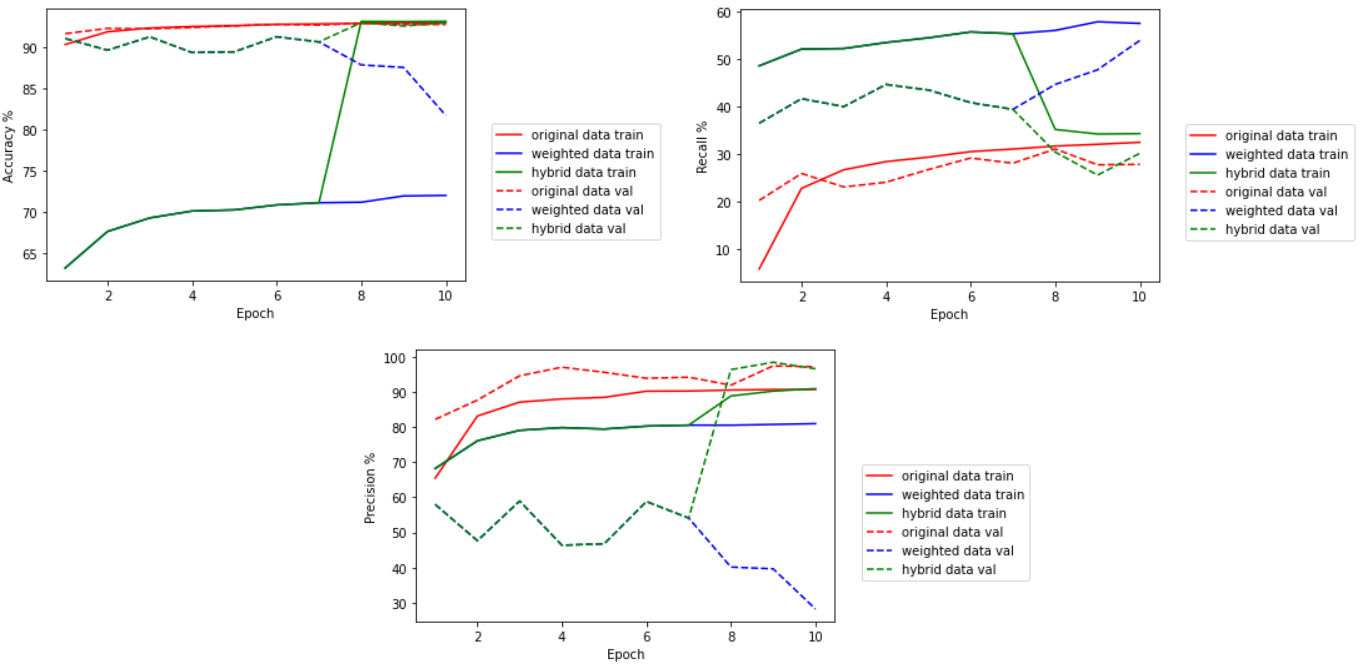
\includegraphics[width=0.9\textwidth]{metrics-acc-recall-prec.png}
\end{figure}
Das Training mit dem original Datensatz hat die höchste Accuracy, allerdings auch den geringsten Recall. Das liegt daran, dass das Modell fast nur darauf trainiert wird 0er Labels zu erkennen und hat daher zwar eine hohe Accuracy, dafür aber einen geringen Recall, da es die meisten 1er Labels nicht als solche interpretiert. Die Precision dagegen ist aber hoch, was bedeutet dass viele der als Signal vorhergesagten Labels auch tatsächlich Signale sind. Da der SETI Datensatz einige Kadenzen aufweist wo die Signale auch mit bloßem Auge gut zu erkennen sind, liegt die Annahme nahe, dass das Modell vor allem die leicht zu findenden Signale erkennt. Ähnlich verhält es sich mit der hybriden Variante, allerdings ist der Recall etwas höher als bei der original Variante. Das liegt daran, dass überwiegend mit einem ausgeglichenem Datensatz trainiert wurde, wodurch das Modell mehr 1er Labels erkennt. Die gewichtete Variante hängt bei der Accuracy und Precision hinterher, dafür ist der Recall bei dieser Variante fast am höchsten, da ausschließlich mit einem augeglichenem Datensatz trainiert wurde. Außerdem ist auffällig dass die Metriken für die Validierungsdaten bei dem ausgeglichenen und hybriden Datensatz von den Metriken der Trainingsdaten abweichen, das hat den Grund dass die Validierungsdaten nicht an das Training angepasst wurden. Validierungsdaten sollten nie verändert werden und insbesondere nicht für das Training eingesetzt werden. Des Weiteren ist auffällig, dass das Training mit den ausgeglichenen Daten zwar eine recht hohe Accuracy und Recall liefert, allerdings leidet die Precision darunter je mehr das Modell gelernt hat. Das hängt unter anderem damit zusammen, dass der Recall immer weiter steigt und das Modell somit immer mehr 1er Labels als Signal interpretiert wobei viele davon gar keine Signale darstellen. Möglicherweise ist das Modell mit welchem trainiert wurde - efficientnet-b1 - nicht komplex genug um diese Aufgabe zu bewältigen. Das lässt sich auch recht gut aus den nächsten Diagrammen herauslesen:
\begin{figure}[h]
\centering
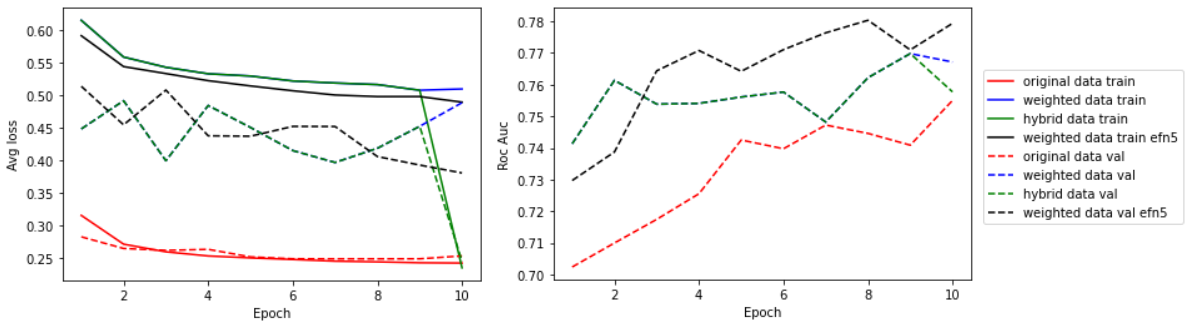
\includegraphics[width=0.9\textwidth]{metrics-avgloss-rocauc.png}
\end{figure}
Am interessantesten ist der Graph mit dem durchschnittlichen Loss. Sowohl bei der hybriden Variante als auch bei der original Variante ist der Loss recht niedrig gegen Ende der Epochen, während der Loss des Modells mit dem ausgeglichenen Datensatz auch am Ende noch recht hoch ist. Das hängt wie oben bereits erwähnt möglicherweise damit zusammen, dass das Modell nicht komplex genug ist. Da viele der Vorhersagen als Signal interpretiert werden, allerdings viele davon auch falsch sind, ist der Loss entsprechend hoch. Der Roc/Auc Score ist bei allen Varianten gegen Ende fast gleich - der Score der gewichteten Variante ist fast am höchsten, da das Verhältnis von Recall und Precision besser ist. Da wie oben bereits angesprochen das Modell efficientnet-b1 möglicherweise nicht komplex genug für die Problematik ist, wurde mit einem komplexeren Modell efficientnet-b5 trainiert und außerdem mit einem ausgeglichenen Datensatz. Die Metriken für das Modell sind in den oben abgebildeten Diagrammen bereits enthalten. Die Verläufe der Metriken ähneln sehr den Verläufen der anderen ausgeglichenen Variante und der hybriden Variante. Allerdings sind die Metriken überwiegend besser, was die Hypothese bestätigt, dass das efficientnet-b5 besser für die Aufgabe geeignet ist als das efficientnet-b1.
\newline
Abschließend kann man sagen, dass sowohl die Variante mit den original Daten als auch die Variante mit den gewichteten Daten beide Vor- und Nachteile haben. Daher ist die hybride Variante ein guter Kompromiss um die Vorteile beider Varianten auszunutzen. Allerdings muss man beim Oversampling aufgepassen, dass das Modell nicht übertrainiert wird auf die mehrfach genutzten Daten. Dabei kann uns Dataaugmentation weiterhelfen.

TODO: Referenz https://arxiv.org/abs/1710.05381

\subsection{Dataugmentation}
Gerade für die Strategie des Oversamplings ist es wichtig aufzupassen, dass das Modell nicht overfittet, also zu sehr auf spezielle Daten trainiert ist und somit auf allgemeinen Daten schlecht abschneidet. Da man beim Oversampling Daten mehrmals für dasselbe Training nutzt ist es sinnvoll die Daten etwas abzuändern, mithilfe von Dataaugmentation. Dabei geht es darum die Daten so zu transformieren, dass sie für das Training immer noch brauchbar sind, aber nicht mehr dem Original entsprechen. Dabei kann das Bild beispielsweise einfach horizontal oder vertikal gespiegelt werden. Es gibt noch viele weitere Möglichkeiten wie Rotieren, das Bild vergrößern und noch einige weitere Varianten. Diese Transformationen geschehen dabei zufällig, also mal wird beispielsweise nur horizontal gespiegelt, mal bleibt das Original erhalten, mal werden alle vorgegebenen Transformationen angewandt. Dadurch erhält man ein komplett neues Bild mit welchem das Modell trainieren kann ohne zu overfitten. Aber Dataaugmentation kann nicht nur sinnvoll sein, wenn man Oversampling angewandt hat, es kann auch sinnvoll sein wenn man ganz normale Trainingsdaten hat und das Modell möglichst breit gefächert auf den Daten lernen lassen möchte. Durch die Transformationen erhält man sozusagen alle möglichen weiteren Szenarien die das Modell erlernen kann.

TODO: Referenz Buch "Deep Learning mit Python und Keras von Francois Chollet"

\subsection{Scheduler}
Trainiert man ein Modell, spielt die Lernrate eine große Rolle, gerade wenn es darum geht die optimalen Parameter zu erhalten. Ist die Lernrate zu klein, dauert es lange bis die optimalen Werte erreicht werden, während bei einer zu hohen Lernrate dieser optimale Punkt übersprungen werden könnte:
\begin{figure}[h]
\centering
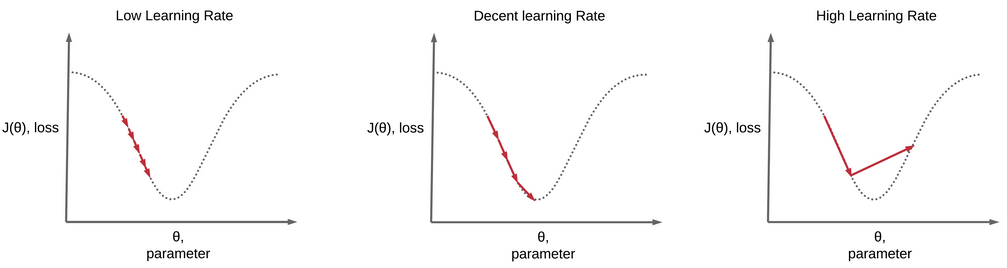
\includegraphics[width=0.9\textwidth]{lernrates-vs.png}
\end{figure}
Ein sogenannter Scheduler kann die Suche nach einer optimalen Lernrate Abhilfe schaffen. Die Grundidee des Schedulers ist die Lernrate über die Epochen hinweg zu verringern. Je höher die Epoche also je mehr man bereits trainiert hat, desto näher ist man am optimalen Punkt und die Lernrate muss immer weiter verringert werden um diesen Punkt nicht zu verpassen. Dadurch erhält man sowohl Vorteile einer hohen Lernrate als auch die Vorteile einer geringen Lernrate: Anfangs ist die Lernrate noch hoch wodurch man sich dem Optimum schnell nähert, aber je näher man dem Optimum näher kommt, desto geringer wird die Lernrate und man veroasst das Optimum nicht.

TODO: Referenz https://www.deeplearningwizard.com/deep_learning/boosting_models_pytorch/lr_scheduling/

\subsection{K Fold Cross Validation}
Wenn man wissen möchte wie gut ein Modell trainiert ist, kann man wie bereits weiter oben erwähnt bestimmte Metriken berechnen lassen, die das Modell bewerten. Dabei kann es rein statistisch gesehen vorkommen, dass das Modell mal besonders schlecht repräsentative Trainingsdaten erhält und somit auf realen Daten schlecht abschneidet. Um robuste Metriken zu berechnen hilft die K Fold Cross Validation. Dabei wird der gesamte Datensatz in k viele Teile unterteilt, wobei es entsprechend k viele Folds gibt. In jedem Fold wird das Modell neu trainiert, allerdings immer wieder mit anderen Trainings- und Validierungsdaten. Die Validierungsdaten beim ersten Fold sind beispielsweise der erste der k Teile, beim zweiten Fold der zweite und so weiter:
\begin{figure}[h]
\centering
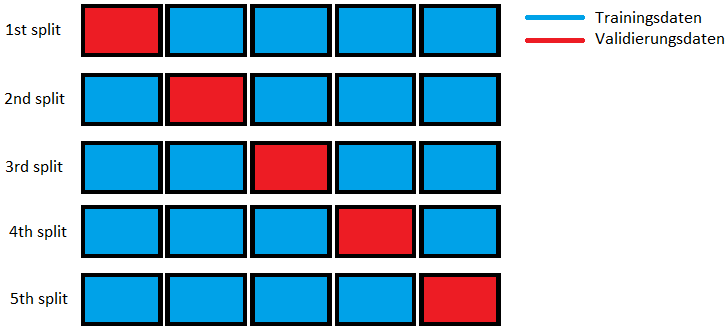
\includegraphics[width=0.9\textwidth]{folds.png}
\end{figure}
Die Metriken können nach Abschluss aller Folds gemittelt werden, wodurch man robuste Werte erhält. Außerdem kann ermittelt werden in welchem Fold das Modell am besten abgeschnitten hat.

TODO: Referenz https://medium.com/dataseries/k-fold-cross-validation-with-pytorch-and-sklearn-d094aa00105f

\section{Tech Stack}
Zusammenfassung der verwendeten Tools und Bibliotheken, die teilweise auch vorher im Text schon genannt wurden.

\section{Fazit}


\end{document}